% 第 19 题四棱锥示意图，虚实线按固定来源第 1 页重绘；坐标仅控制图形布局。
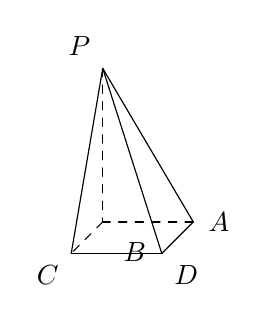
\begin{tikzpicture}[x=1cm,y=1cm,line width=0.42pt,line cap=round,line join=round]
  \coordinate (B) at (0,0);
  \coordinate (A) at (1.15,0);
  \coordinate (C) at (-0.40,-0.40);
  \coordinate (D) at (0.75,-0.40);
  \coordinate (P) at (0,1.95);

  % 虚线：PB、AB、BC。
  \draw[dashed] (P) -- (B);
  \draw[dashed] (A) -- (B);
  \draw[dashed] (B) -- (C);

  % 实线：PA、PC、PD、AD、CD。
  \draw (P) -- (A);
  \draw (P) -- (C);
  \draw (P) -- (D);
  \draw (A) -- (D);
  \draw (C) -- (D);

  \node[above left=1pt] at (P) {$P$};
  \node[right=2pt] at (A) {$A$};
  \node[below right=4pt] at (B) {$B$};
  \node[below left=1pt] at (C) {$C$};
  \node[below right=1pt] at (D) {$D$};
\end{tikzpicture}
